\documentclass[12pt]{article}
%Fall 2022
% Some basic packages
\usepackage{standalone}[subpreambles=true]
\usepackage[utf8]{inputenc}
\usepackage[T1]{fontenc}
\usepackage{textcomp}
\usepackage[english]{babel}
\usepackage{url}
\usepackage{graphicx}
%\usepackage{quiver}
\usepackage{float}
\usepackage{enumitem}
\usepackage{lmodern}
\usepackage{comment}
\usepackage{hyperref}
\usepackage[usenames,svgnames,dvipsnames]{xcolor}
\usepackage[margin=1in]{geometry}
\usepackage{pdfpages}

\pdfminorversion=7

% Don't indent paragraphs, leave some space between them
\usepackage{parskip}

% Hide page number when page is empty
\usepackage{emptypage}
\usepackage{subcaption}
\usepackage{multicol}
\usepackage[b]{esvect}

% Math stuff
\usepackage{amsmath, amsfonts, mathtools, amsthm, amssymb}
\usepackage{bbm}
\usepackage{stmaryrd}
\allowdisplaybreaks

% Fancy script capitals
\usepackage{mathrsfs}
\usepackage{cancel}
% Bold math
\usepackage{bm}
% Some shortcuts
\newcommand{\rr}{\ensuremath{\mathbb{R}}}
\newcommand{\zz}{\ensuremath{\mathbb{Z}}}
\newcommand{\qq}{\ensuremath{\mathbb{Q}}}
\newcommand{\nn}{\ensuremath{\mathbb{N}}}
\newcommand{\ff}{\ensuremath{\mathbb{F}}}
\newcommand{\cc}{\ensuremath{\mathbb{C}}}
\newcommand{\ee}{\ensuremath{\mathbb{E}}}
\newcommand{\hh}{\ensuremath{\mathbb{H}}}
\renewcommand\O{\ensuremath{\emptyset}}
\newcommand{\norm}[1]{{\left\lVert{#1}\right\rVert}}
\newcommand{\dbracket}[1]{{\left\llbracket{#1}\right\rrbracket}}
\newcommand{\ve}[1]{{\bm{#1}}}
\newcommand\allbold[1]{{\boldmath\textbf{#1}}}
\DeclareMathOperator{\lcm}{lcm}
\DeclareMathOperator{\im}{im}
\DeclareMathOperator{\coim}{coim}
\DeclareMathOperator{\dom}{dom}
\DeclareMathOperator{\tr}{tr}
\DeclareMathOperator{\rank}{rank}
\DeclareMathOperator*{\var}{Var}
\DeclareMathOperator*{\ev}{E}
\DeclareMathOperator{\dg}{deg}
\DeclareMathOperator{\aff}{aff}
\DeclareMathOperator{\conv}{conv}
\DeclareMathOperator{\inte}{int}
\DeclareMathOperator*{\argmin}{argmin}
\DeclareMathOperator*{\argmax}{argmax}
\DeclareMathOperator{\graph}{graph}
\DeclareMathOperator{\sgn}{sgn}
\DeclareMathOperator*{\Rep}{Rep}
\DeclareMathOperator{\Proj}{Proj}
\DeclareMathOperator{\mat}{mat}
\DeclareMathOperator{\diag}{diag}
\DeclareMathOperator{\aut}{Aut}
\DeclareMathOperator{\gal}{Gal}
\DeclareMathOperator{\inn}{Inn}
\DeclareMathOperator{\edm}{End}
\DeclareMathOperator{\Hom}{Hom}
\DeclareMathOperator{\ext}{Ext}
\DeclareMathOperator{\tor}{Tor}
\DeclareMathOperator{\Span}{Span}
\DeclareMathOperator{\Stab}{Stab}
\DeclareMathOperator{\cont}{cont}
\DeclareMathOperator{\Ann}{Ann}
\DeclareMathOperator{\Div}{div}
\DeclareMathOperator{\curl}{curl}
\DeclareMathOperator{\nat}{Nat}
\DeclareMathOperator{\gr}{Gr}
\DeclareMathOperator{\vect}{Vect}
\DeclareMathOperator{\id}{id}
\DeclareMathOperator{\Mod}{Mod}
\DeclareMathOperator{\sign}{sign}
\DeclareMathOperator{\Surf}{Surf}
\DeclareMathOperator{\fcone}{fcone}
\DeclareMathOperator{\Rot}{Rot}
\DeclareMathOperator{\grad}{grad}
\DeclareMathOperator{\atan2}{atan2}
\DeclareMathOperator{\Ric}{Ric}
\let\vec\relax
\DeclareMathOperator{\vec}{vec}
\let\Re\relax
\DeclareMathOperator{\Re}{Re}
\let\Im\relax
\DeclareMathOperator{\Im}{Im}
% Put x \to \infty below \lim
\let\svlim\lim\def\lim{\svlim\limits}

%wide hat
\usepackage{scalerel,stackengine}
\stackMath
\newcommand*\wh[1]{%
\savestack{\tmpbox}{\stretchto{%
  \scaleto{%
    \scalerel*[\widthof{\ensuremath{#1}}]{\kern-.6pt\bigwedge\kern-.6pt}%
    {\rule[-\textheight/2]{1ex}{\textheight}}%WIDTH-LIMITED BIG WEDGE
  }{\textheight}% 
}{0.5ex}}%
\stackon[1pt]{#1}{\tmpbox}%
}
\parskip 1ex

%Make implies and impliedby shorter
\let\implies\Rightarrow
\let\impliedby\Leftarrow
\let\iff\Leftrightarrow
\let\epsilon\varepsilon

% Add \contra symbol to denote contradiction
\usepackage{stmaryrd} % for \lightning
\newcommand\contra{\scalebox{1.5}{$\lightning$}}

% \let\phi\varphi

% Command for short corrections
% Usage: 1+1=\correct{3}{2}

\definecolor{correct}{HTML}{009900}
\newcommand\correct[2]{\ensuremath{\:}{\color{red}{#1}}\ensuremath{\to }{\color{correct}{#2}}\ensuremath{\:}}
\newcommand\green[1]{{\color{correct}{#1}}}

% horizontal rule
\newcommand\hr{
    \noindent\rule[0.5ex]{\linewidth}{0.5pt}
}

% hide parts
\newcommand\hide[1]{}

% si unitx
\usepackage{siunitx}
\sisetup{locale = FR}

%allows pmatrix to stretch
\makeatletter
\renewcommand*\env@matrix[1][\arraystretch]{%
  \edef\arraystretch{#1}%
  \hskip -\arraycolsep
  \let\@ifnextchar\new@ifnextchar
  \array{*\c@MaxMatrixCols c}}
\makeatother

\renewcommand{\arraystretch}{0.8}

\renewcommand{\baselinestretch}{1.5}

\usepackage{graphics}
\usepackage{epstopdf}

\RequirePackage{hyperref}
%%
%% Add support for color in order to color the hyperlinks.
%% 
\hypersetup{
  colorlinks = true,
  urlcolor = blue,
  citecolor = blue
}
%%fakesection Links
\hypersetup{
    colorlinks,
    linkcolor={red!50!black},
    citecolor={green!50!black},
    urlcolor={blue!80!black}
}
%customization of cleveref
\RequirePackage[capitalize,nameinlink]{cleveref}[0.19]

% Per SIAM Style Manual, "section" should be lowercase
\crefname{section}{section}{sections}
\crefname{subsection}{subsection}{subsections}
\Crefname{section}{Section}{Sections}
\Crefname{subsection}{Subsection}{Subsections}

% Per SIAM Style Manual, "Figure" should be spelled out in references
\Crefname{figure}{Figure}{Figures}

% Per SIAM Style Manual, don't say equation in front on an equation.
\crefformat{equation}{\textup{#2(#1)#3}}
\crefrangeformat{equation}{\textup{#3(#1)#4--#5(#2)#6}}
\crefmultiformat{equation}{\textup{#2(#1)#3}}{ and \textup{#2(#1)#3}}
{, \textup{#2(#1)#3}}{, and \textup{#2(#1)#3}}
\crefrangemultiformat{equation}{\textup{#3(#1)#4--#5(#2)#6}}%
{ and \textup{#3(#1)#4--#5(#2)#6}}{, \textup{#3(#1)#4--#5(#2)#6}}{, and \textup{#3(#1)#4--#5(#2)#6}}

% But spell it out at the beginning of a sentence.
\Crefformat{equation}{#2Equation~\textup{(#1)}#3}
\Crefrangeformat{equation}{Equations~\textup{#3(#1)#4--#5(#2)#6}}
\Crefmultiformat{equation}{Equations~\textup{#2(#1)#3}}{ and \textup{#2(#1)#3}}
{, \textup{#2(#1)#3}}{, and \textup{#2(#1)#3}}
\Crefrangemultiformat{equation}{Equations~\textup{#3(#1)#4--#5(#2)#6}}%
{ and \textup{#3(#1)#4--#5(#2)#6}}{, \textup{#3(#1)#4--#5(#2)#6}}{, and \textup{#3(#1)#4--#5(#2)#6}}

% Make number non-italic in any environment.
\crefdefaultlabelformat{#2\textup{#1}#3}

% Environments
\makeatother
% For box around Definition, Theorem, \ldots
%%fakesection Theorems
\usepackage{thmtools}
\usepackage[framemethod=TikZ]{mdframed}

\theoremstyle{definition}
\mdfdefinestyle{mdbluebox}{%
	roundcorner = 10pt,
	linewidth=1pt,
	skipabove=12pt,
	innerbottommargin=9pt,
	skipbelow=2pt,
	nobreak=true,
	linecolor=blue,
	backgroundcolor=TealBlue!5,
}
\declaretheoremstyle[
	headfont=\sffamily\bfseries\color{MidnightBlue},
	mdframed={style=mdbluebox},
	headpunct={\\[3pt]},
	postheadspace={0pt}
]{thmbluebox}

\mdfdefinestyle{mdredbox}{%
	linewidth=0.5pt,
	skipabove=12pt,
	frametitleaboveskip=5pt,
	frametitlebelowskip=0pt,
	skipbelow=2pt,
	frametitlefont=\bfseries,
	innertopmargin=4pt,
	innerbottommargin=8pt,
	nobreak=false,
	linecolor=RawSienna,
	backgroundcolor=Salmon!5,
}
\declaretheoremstyle[
	headfont=\bfseries\color{RawSienna},
	mdframed={style=mdredbox},
	headpunct={\\[3pt]},
	postheadspace={0pt},
]{thmredbox}

\declaretheorem[%
style=thmbluebox,name=Theorem,numberwithin=section]{thm}
\declaretheorem[style=thmbluebox,name=Lemma,sibling=thm]{lem}
\declaretheorem[style=thmbluebox,name=Proposition,sibling=thm]{prop}
\declaretheorem[style=thmbluebox,name=Corollary,sibling=thm]{coro}
\declaretheorem[style=thmredbox,name=Example,sibling=thm]{eg}

\mdfdefinestyle{mdgreenbox}{%
	roundcorner = 10pt,
	linewidth=1pt,
	skipabove=12pt,
	innerbottommargin=9pt,
	skipbelow=2pt,
	nobreak=true,
	linecolor=ForestGreen,
	backgroundcolor=ForestGreen!5,
}

\declaretheoremstyle[
	headfont=\bfseries\sffamily\color{ForestGreen!70!black},
	bodyfont=\normalfont,
	spaceabove=2pt,
	spacebelow=1pt,
	mdframed={style=mdgreenbox},
	headpunct={ --- },
]{thmgreenbox}

\declaretheorem[style=thmgreenbox,name=Definition,sibling=thm]{defn}

\mdfdefinestyle{mdgreenboxsq}{%
	linewidth=1pt,
	skipabove=12pt,
	innerbottommargin=9pt,
	skipbelow=2pt,
	nobreak=true,
	linecolor=ForestGreen,
	backgroundcolor=ForestGreen!5,
}
\declaretheoremstyle[
	headfont=\bfseries\sffamily\color{ForestGreen!70!black},
	bodyfont=\normalfont,
	spaceabove=2pt,
	spacebelow=1pt,
	mdframed={style=mdgreenboxsq},
	headpunct={},
]{thmgreenboxsq}
\declaretheoremstyle[
	headfont=\bfseries\sffamily\color{ForestGreen!70!black},
	bodyfont=\normalfont,
	spaceabove=2pt,
	spacebelow=1pt,
	mdframed={style=mdgreenboxsq},
	headpunct={},
]{thmgreenboxsq*}

\mdfdefinestyle{mdblackbox}{%
	skipabove=8pt,
	linewidth=3pt,
	rightline=false,
	leftline=true,
	topline=false,
	bottomline=false,
	linecolor=black,
	backgroundcolor=RedViolet!5!gray!5,
}
\declaretheoremstyle[
	headfont=\bfseries,
	bodyfont=\normalfont\small,
	spaceabove=0pt,
	spacebelow=0pt,
	mdframed={style=mdblackbox}
]{thmblackbox}

\theoremstyle{plain}
\declaretheorem[name=Question,sibling=thm,style=thmblackbox]{ques}
\declaretheorem[name=Remark,sibling=thm,style=thmgreenboxsq]{remark}
\declaretheorem[name=Remark,sibling=thm,style=thmgreenboxsq*]{remark*}
\newtheorem{ass}[thm]{Assumptions}

\theoremstyle{definition}
\newtheorem*{problem}{Problem}
\newtheorem{claim}[thm]{Claim}
\theoremstyle{remark}
\newtheorem*{case}{Case}
\newtheorem*{notation}{Notation}
\newtheorem*{note}{Note}
\newtheorem*{motivation}{Motivation}
\newtheorem*{intuition}{Intuition}
\newtheorem*{conjecture}{Conjecture}

% Make section starts with 1 for report type
%\renewcommand\thesection{\arabic{section}}

% End example and intermezzo environments with a small diamond (just like proof
% environments end with a small square)
\usepackage{etoolbox}
\AtEndEnvironment{vb}{\null\hfill$\diamond$}%
\AtEndEnvironment{intermezzo}{\null\hfill$\diamond$}%
% \AtEndEnvironment{opmerking}{\null\hfill$\diamond$}%

% Fix some spacing
% http://tex.stackexchange.com/questions/22119/how-can-i-change-the-spacing-before-theorems-with-amsthm
\makeatletter
\def\thm@space@setup{%
  \thm@preskip=\parskip \thm@postskip=0pt
}

% Fix some stuff
% %http://tex.stackexchange.com/questions/76273/multiple-pdfs-with-page-group-included-in-a-single-page-warning
\pdfsuppresswarningpagegroup=1


% My name
\author{Jaden Wang}



\begin{document}
\centerline {\textsf{\textbf{\LARGE{Homework 4}}}}
\centerline {Jaden Wang}
\vspace{.15in}
Consider the following figure:
~\begin{figure}[H]
	\centering
	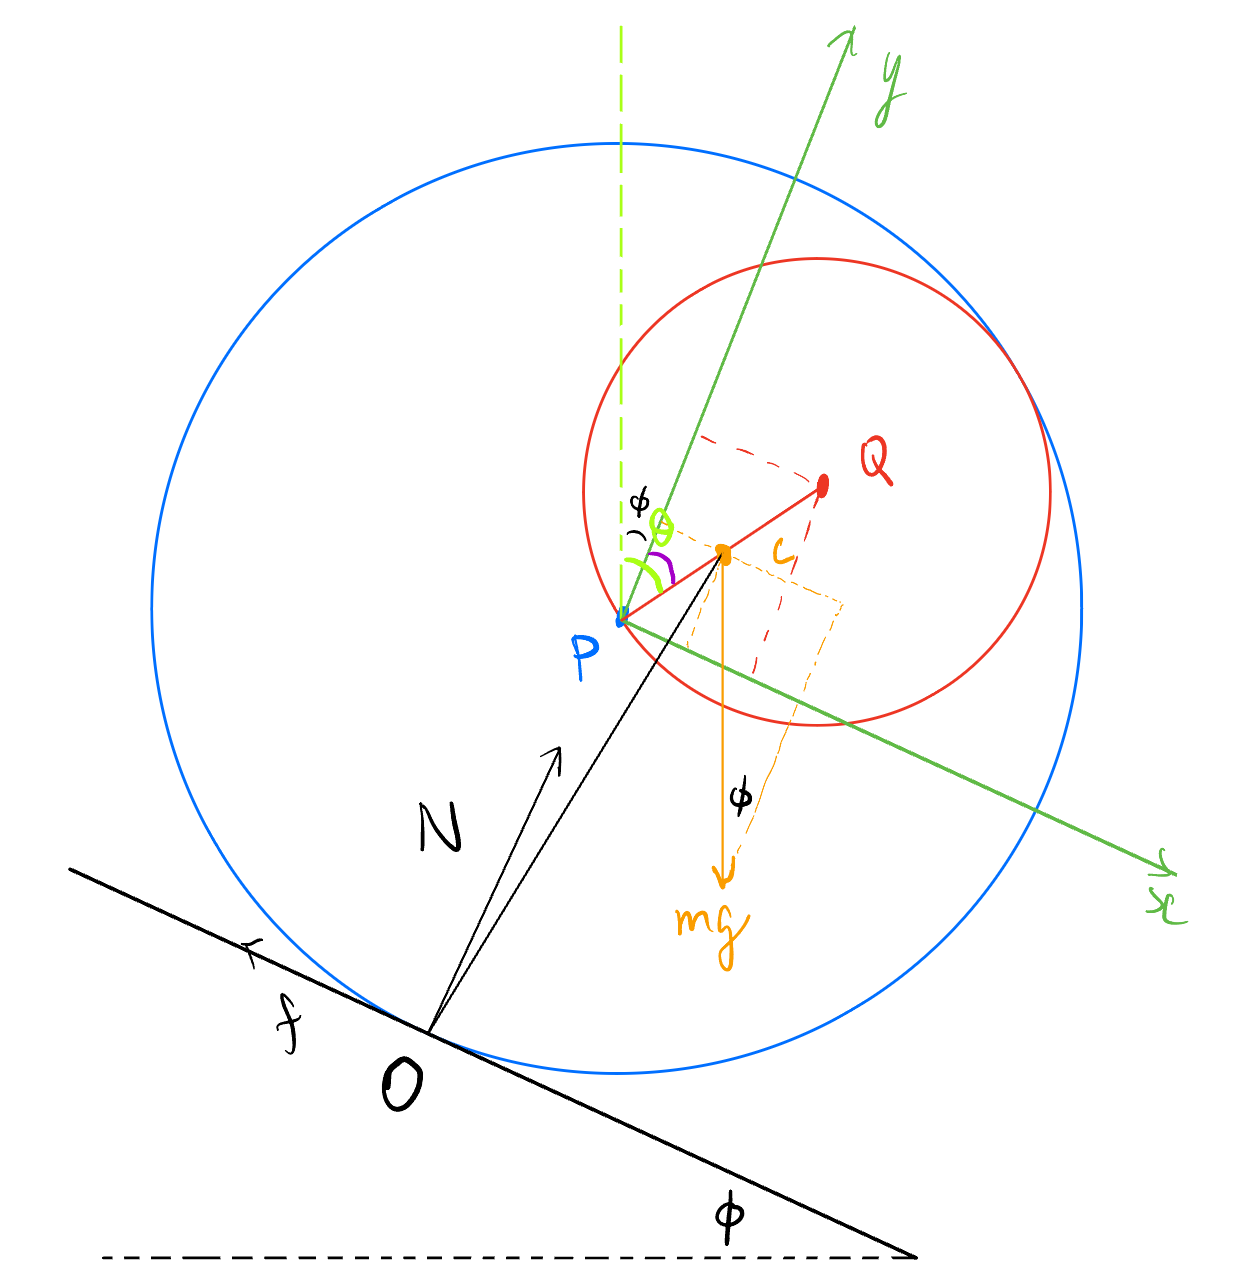
\includegraphics[width=0.6\textwidth]{./figures/hw4.1.png}
\end{figure}
Take $ P$ as the coordinate origin and let  $ Q$ be the center of mass of the red cylinder,  $ \frac{R}{2}$ apart from $ P$. To compute the center of mass, we can simplify the problem by patching the hole of the blue cylinder uniformly via giving  $ \rho$ worth of mass from the red cylinder so the blue becomes a perfect cylinder with center of mass  $ P$. Then the red cylinder has  $ 4 \rho$ worth of mass left with center of mass still at $ Q$. From now on, we refer to this patched blue cylinder as blue and the reduced red as red. Then we have $ m_b = \pi R^2 \rho$, $ m_r = \pi\left( \frac{R}{2} \right) ^2 4 \rho = \pi R^2 \rho = m_b$, $ m = m_b + m_r = 2 \pi R^2 \rho$ and
\begin{align*}
	r_C &= \frac{1}{m} (m_b r_b + m_r r_r) \\
	    &=\frac{\pi R^2 \rho \left(  0 + \frac{R}{2}\right) }{ m}\\ 
	    &= \frac{R}{4} .
\end{align*}
So the center of mass is exactly halfway between $ PQ$. Since we know the moment of inertia of a cylinder about its center of mass is $I = \frac{1}{2} mR^2$, and $ P$ is the center of mass of blue, we compute $ I_C^{b} = I_P^{b} = \frac{1}{2} m_b R^2$, $ I_C^r = \frac{1}{2} m_r \left( \frac{R}{2} \right) ^2 = \frac{1}{8} m_r R^2$, $ I_P^{r} = I_C^{r} + m_r \left( \frac{R}{2} \right) ^2 = \frac{3}{8}m_rR^2$ by parallel axis theorem. Thus we have
\begin{align*}
	I_p = I_p^b + I_p^r =\frac{1}{2}m_bR^2 + \frac{3}{8}m_rR^2 = \frac{7}{16} mR^2.
\end{align*}
Parallel axis theorem gives
\begin{align*}
	I_C &= I_p - m\left( \frac{R}{4} \right)^2  \\
	&= \left( \frac{7}{16}-\frac{1}{16} \right) mR^2 \\
	&= \frac{3}{8}mR^2 
\end{align*}

Now let us consider the frictionless case, which necessarily slips because there is no friction to counter the $ x$-direction motion at $ O$. Considering the entire cylinder, we see that in the $ x$-direction the only net force comes from gravity, so by Euler's first law,
 \begin{align*}
	m\ddot{x}_C = F_{net}^{x} = mg \sin\phi.
\end{align*}
In the $ y$-direction, we have 
\begin{align*}
	m\ddot{y}_C = F_{net}^{y} = N - mg \cos \phi .
\end{align*}
Now consider the cylinder as two separate cylinders. The patched blue one has center of mass $ P$ and has no net force in the  $ y$-direction since $ y_p = 0$ at all times. The reduced red one has center of mass $ Q$ and remains fixed in the body frame $ B$ of the cylinder. Since we are only considering $ y$-direction, the translation in  $ x$-direction is ignored so we are exactly in the scenario of a rotating frame about $ P$ which is fixed in inertia frame in the  $ y$-direction. Then Newton's 2nd law yields
\begin{align*}
     \ve{F}_{net}^B = m \ddot{\ve{r}}^B = \ve{F}_{net}^I + \underbrace{m\ve{\Omega} \times (\ve{r} \times \ve{\Omega})}_{\text{centrifugal force}} + \underbrace{2 m ( \dot{\ve{r}}^B \times \ve{\Omega} )}_{\text{Coriolis force}} + \underbrace{m \ve{r} \times \dot{\ve{\Omega}}^I}_{\text{Euler force}}, 
\end{align*}
where $ \ve{ \Omega} = \dot{\theta} \wh{ z}$ and $ \ve{ r} = \ve{ r}^{PQ}$. Since $ Q$ is fixed in the body frame, it experiences no net force in $ B$ and no Coriolis force, it follows that the net force experienced by the reduced red cylinder in the $ y$-direction (with respect to the inertia frame) is
\begin{align*}
	F_r = - m_r \dot{\theta}^2 \frac{R}{2} \cos \phi + m_r \frac{R}{2} \sin \phi \dot{\theta} .
\end{align*}
By Euler's 1st law, we have
\begin{align*}
	m \ddot{y}_C &= F_b + F_r \\
	&= - \frac{1}{2}m \dot{\theta}^2 \frac{R}{2} \cos \phi + \frac{1}{2}m \frac{R}{2} \sin \phi \dot{\theta} 
\end{align*}
Note that the given data use the opposite orientation for angular stuff, so we have to reverse the sign in the 2nd term in the code (and many other places in the upcoming equations).

Now, Euler's 2nd law says
\begin{align*}
	I_C \ddot{\theta} \wh{ z}&= \ve{ r}^{CO} \times  N \wh{ y}   \\
	&= \begin{pmatrix} -\frac{R}{4} \sin(\theta-\phi) \\ -R-\frac{R}{4} \cos(\theta-\phi)\\0 \end{pmatrix} \times   \begin{pmatrix} 0\\N\\0 \end{pmatrix} \\
	I_C \ddot{\theta}&=- \frac{NR}{4} \sin(\theta - \phi) .
\end{align*}
Here we need to switch sign in the code too. Thus we obtain a system of equations
\begin{align*}
\begin{cases}
	\ddot{x}_C = g \sin\phi\\
	\ddot{y}_C = N - mg \cos \phi \\
	\ddot{y}_C = - \frac{1}{2}\dot{\theta}^2 \frac{R}{2} \cos \phi - \frac{1}{2}\frac{R}{2} \sin \phi \dot{\theta} \\
	I_C \ddot{\theta} =-\frac{NR}{4} \sin(\theta - \phi) 
\end{cases}
\end{align*}
Solving these 4 equations with 4 unknowns yields exactly the validation results.


Now, consider the case of slipping with friction, and the friction coefficient $ \mu = 0.1$. This means the friction is $ \ve{ f}  = -f \wh{ x} = - \mu N \wh{ x}$. Moreover, we have additional torque from the friction, therefore
\begin{align*}
	I_C \ddot{\theta} \wh{ z} &=\ve{ r}^{CO} \times  (-f \wh{ x} + N \wh{ y}) \\
	&= \begin{pmatrix} -\frac{R}{4} \sin(\theta-\phi) \\ -R-\frac{R}{4} \cos(\theta-\phi)\\0 \end{pmatrix} \times   \begin{pmatrix} -f\\N\\0 \end{pmatrix} \\
	-I_C \ddot{\theta} &= \frac{NR}{4} \sin(\theta - \phi) + \left( \frac{R}{4} \cos(\theta - \phi) +R \right) f .
\end{align*}
Again we need to remember to switch signs in the code. Thus the system of equations becomes
\begin{align*}
\begin{cases}
	\ddot{x}_C = mg \sin\phi-f\\
	\ddot{y}_C = N - mg \cos \phi \\
	m \ddot{y}_C = - \frac{1}{2}m \dot{\theta}^2 \frac{R}{2} \cos \phi + \frac{1}{2}m \frac{R}{2} \sin \phi \dot{\theta} \\
	I_C \ddot{\theta} = \frac{NR}{4} \sin(\theta - \phi) + \left( \frac{R}{4} \cos(\theta - \phi) +R \right) f \\
	f = \mu N
\end{cases}
\end{align*}
The results again match the validation data.

Finally, we consider the case of rolling. In this case, the point of contact $ O$ must have zero velocity to not slip. But since we still have rotational motion $ v_o = v_p + R \dot{\theta}$, this yields $ v_p = - R \dot{\theta}$ and $ a_p = -R \ddot{\theta}$. Moreover, since $ PO$ is always perpendicular to the  $ x$-axis, the acceleration is entirely in the  $ x$-direction, \emph{i.e.} $ \ve{ a}_p = a_p \wh{ x} $. To obtain the acceleration of $ C$, we are in the case of two points fixed in the body frame, so we simply apply the formula
 \begin{align*}
	 ^I\ve{ a}_C &= \ ^I \ve{ a}_p + \ ^I\ve{ \Omega }^B \times \ ^I\ve{\Omega}^B \times \ve{ r}^{PC} +\ ^I\dot{\ve{ \Omega}}^B \times \ve{ r}^{PC}  \\
		       &=\ ^I \ve{ a}_p + \begin{pmatrix} 0\\0\\ \dot{\theta} \end{pmatrix}  \times \begin{pmatrix} 0\\0\\ \dot{\theta} \end{pmatrix} \times \begin{pmatrix} \frac{R}{4} \sin(\theta - \phi) \\ \frac{R}{4} \cos(\theta-\phi)\\0 \end{pmatrix} + \begin{pmatrix} 0\\0\\ \ddot{\theta} \end{pmatrix} \times \begin{pmatrix} \frac{R}{4} \sin(\theta - \phi) \\ \frac{R}{4} \cos(\theta-\phi)\\0 \end{pmatrix}  \\
		      \ddot{x}_C &= -R \ddot{\theta} - \frac{R}{4} \left( \ddot{\theta} \cos(\theta - \phi) - \dot{\theta}^2 \sin(\theta - \phi) \right)  
\end{align*}
Again we need to reverse the sign whenever we see an odd power of $ \dot{\theta}$ or $ \ddot{\theta}$ in the code. Thus we obtain the system of equations
\begin{align*}
\begin{cases}
	\ddot{x}_C = mg \sin\phi-f\\
	\ddot{y}_C = N - mg \cos \phi \\
	m \ddot{y}_C = - \frac{1}{2}m \dot{\theta}^2 \frac{R}{2} \cos \phi + \frac{1}{2}m \frac{R}{2} \sin \phi \dot{\theta} \\
	-I_C \ddot{\theta} = \frac{NR}{4} \sin(\theta - \phi) + \left( \frac{R}{4} \cos(\theta - \phi) +R \right) f \\
	\ddot{x}_C = -R \ddot{\theta} - \frac{R}{4} \left( \ddot{\theta} \cos(\theta - \phi) - \dot{\theta}^2 \sin(\theta - \phi) \right).
\end{cases}
\end{align*}
Again the results match!
\end{document}
